\chapter{Starting point}\label{chapter:starting-point}
Before moving to an in-depth analysis of what we realized, it is important to understand the starting point from which the idea of such a project was born.
ECLAIR is already widely used in many contexts in which static analysis is mandatory and enforced by standard regulations. Currently, the developers run ECLAIR on their desktop through a GUI or a CLI. 
\begin{figure}[ht]
	\centering
	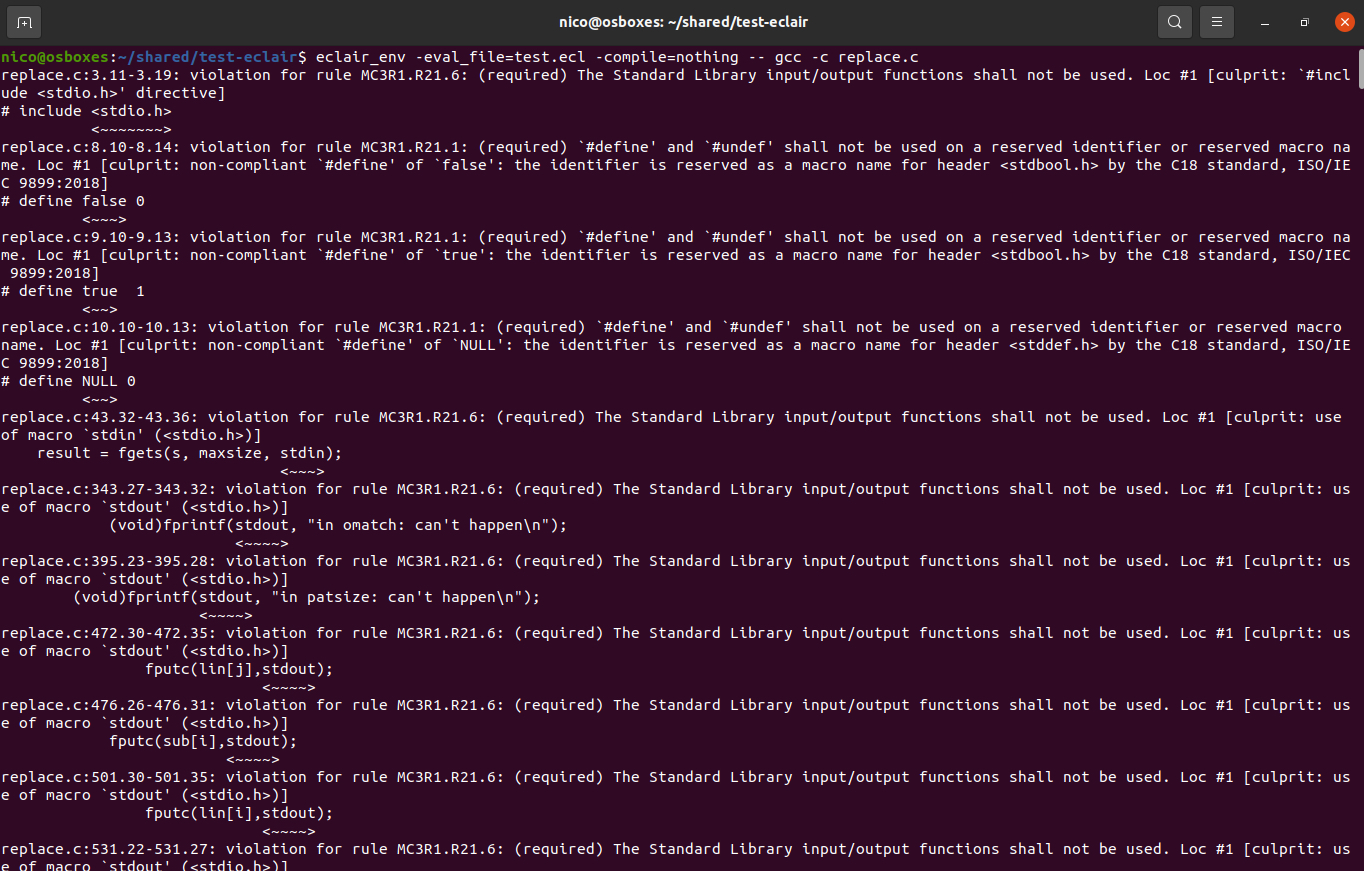
\includegraphics[width=1\textwidth]{Immagini/eclair_cli.jpg}
	\caption{ECLAIR CLI}
	\label{fig:one}
\end{figure}

In particular the first step in ECLAIR setup is configuring the toolchain, that means to indicate installed tools such as compilers and linkers: this is required since the kind of analysis that is performed is bound to the way the software is compiled. 

In addition, ECLAIR needs a \emph{.ecl} file in which rules can be activated or disabled and the report format is specified. 

\begin{lstlisting}[caption={Example \emph{.ecl} file}, label={lst:block_struct}]
-project_root=getenv(``ECLAIR_PROJECT_ROOT")

-enable=B.REPORT.TXT
-enable=MC3R1.R
-disable=`sav&&!B'
# -enable=MC3R1.R8.13

-frames={hide,`kind(object||program||project)'}

# Hides all reports that have all areas external to project root tree.
-reports+={hide,all_exp_external}
\end{lstlisting}

After the analysis, ECLAIR can produce different kinds of outputs:
\begin{itemize}
  \item summary outputs, which contain comprehensive information about the analysis, as well as counts of the issues uncovered by the analysis per service, per file, per tag and combinations;
  \item rich outputs, which contain comprehensive information about the analysis results without going into the detail of each reported program condition;
  \item detailed outputs, which contain comprehensive information about the analysis results, including all details about each reported program condition (such as a coding rule violation or a possible run-time error) and all the information required for a proper understanding of each individual issue reported by the analysis;
  \item metric outputs, which contain the values of the metrics collected for each file, function and project.
\end{itemize}

These outputs can be returned in different formats:
\begin{itemize}
  \item summary and rich outputs in printable format (\emph{.odt} or \emph{.doc}), HTML format or pure text;
  \item rich interactive outputs in spreadsheet format, which contain the set of ECLAIR findings in a form that is suitable for the communication to third parties that are only interested in the residual violations and whether they have been justified and how;
  \item detailed outputs in interactive spreadsheet format, pure text format or printable format.
\end{itemize}

\begin{figure}[ht]
	\centering
	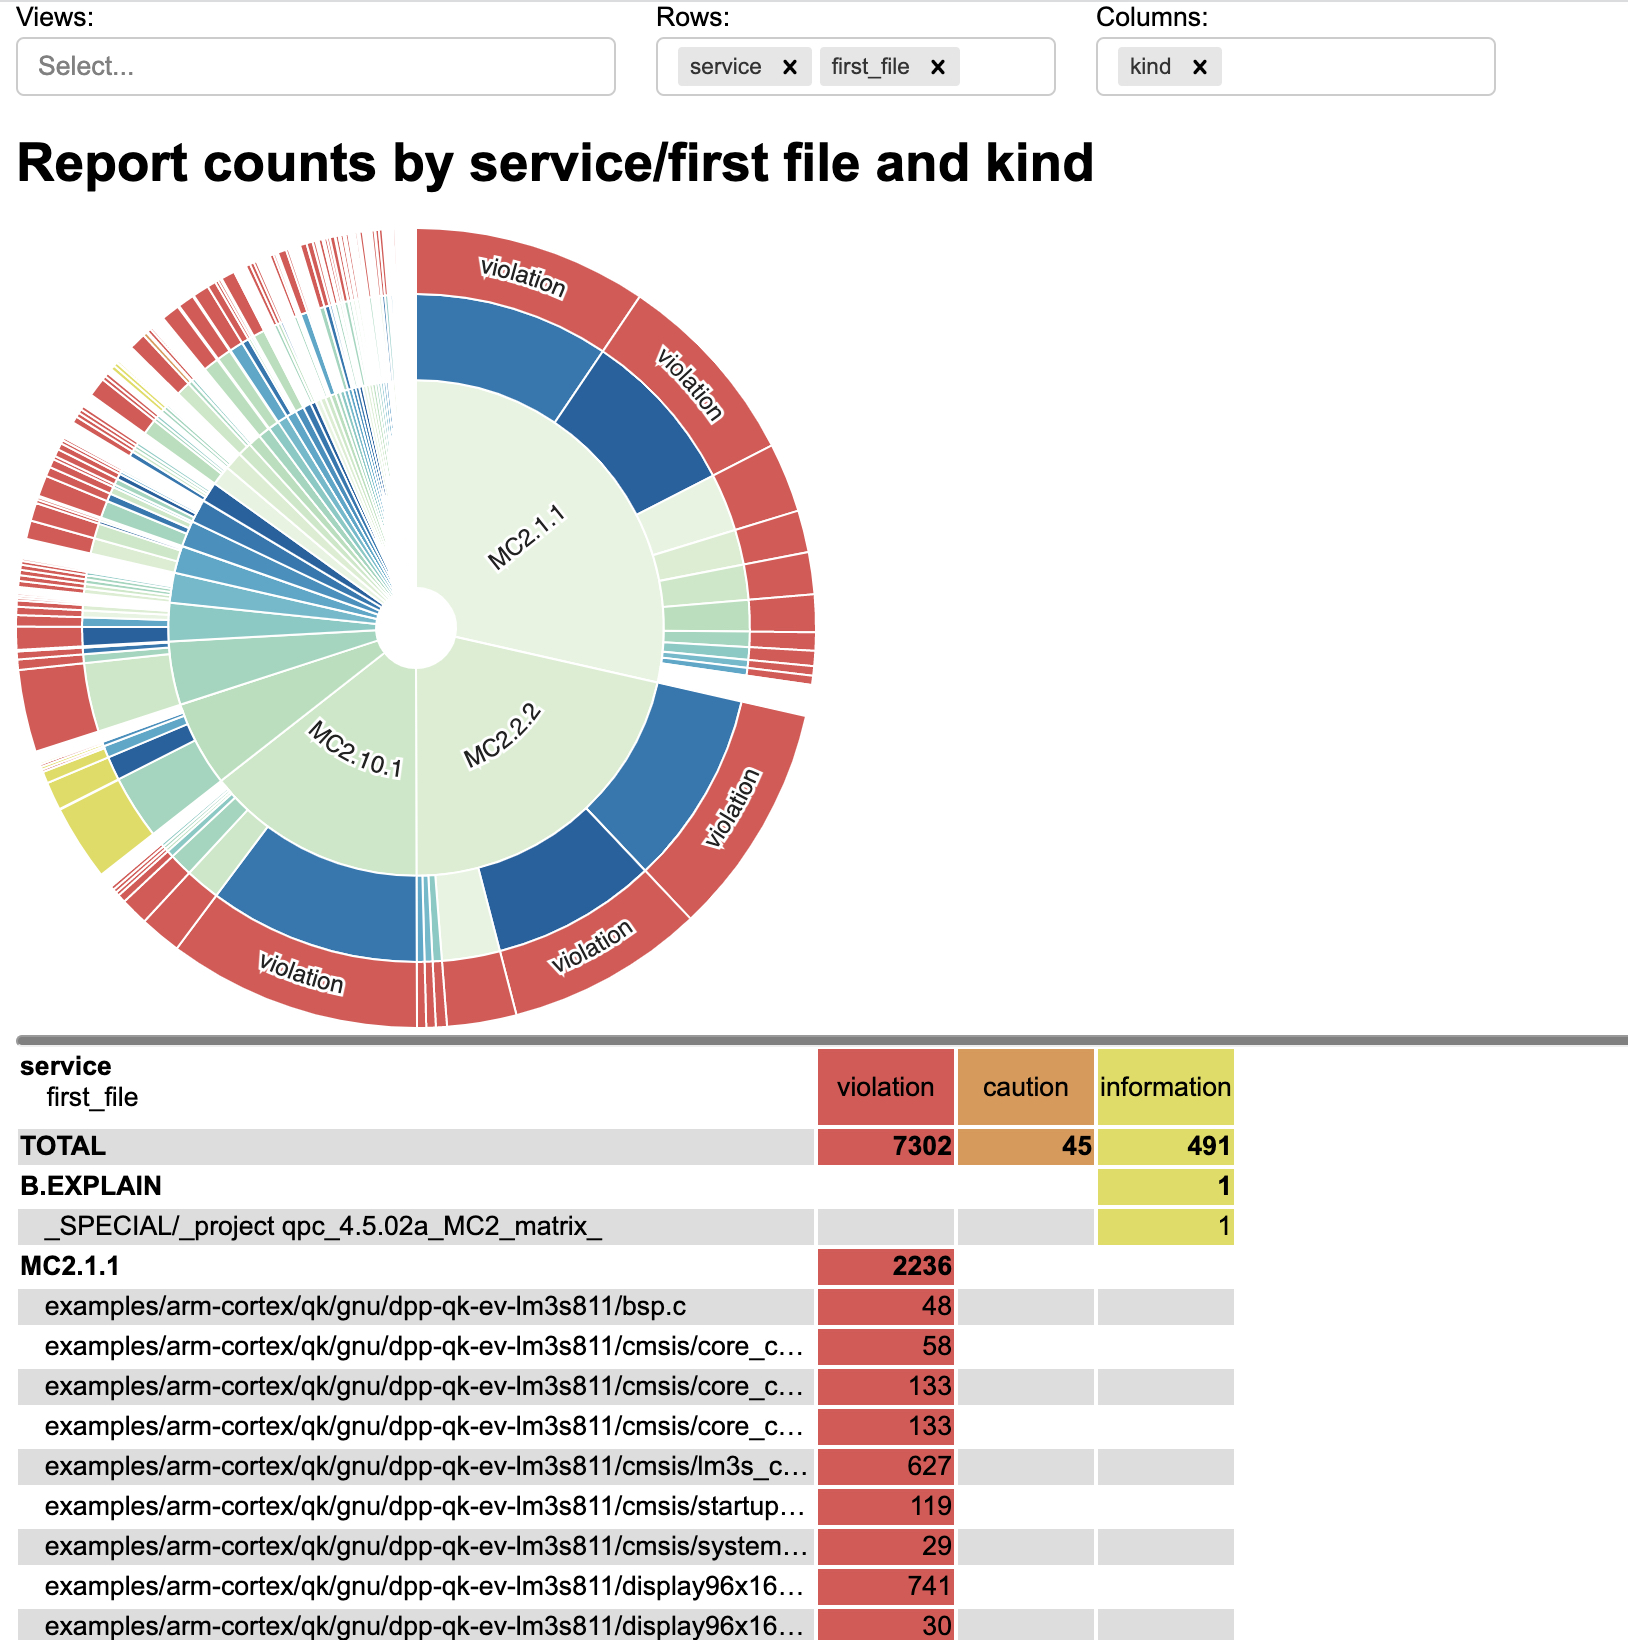
\includegraphics[width=1\textwidth]{Immagini/eclair_rich_output_html.jpg}
	\caption{Example of ECLAIR rich output in HTML format}
	\label{fig:one}
\end{figure}

Since static analysis integration in continuous integration pipelines is a must-have in modern development, the eclairit.com web site was created. This demonstrates the use of ECLAIR integrated into Jenkins\footnote{https://www.jenkins.io} and GitLab. An integration server performs the analysis and provides the reports directly in the browser, without having to install ECLAIR on each PC. This was the first change of paradigm from the traditional analysis performed directly on developers' machines.
This tool gave us the inspiration to integrate ECLAIR in the development workflow in a new way: we wanted to perform the analysis while the users were writing the code.

\begin{figure}[ht]
	\centering
	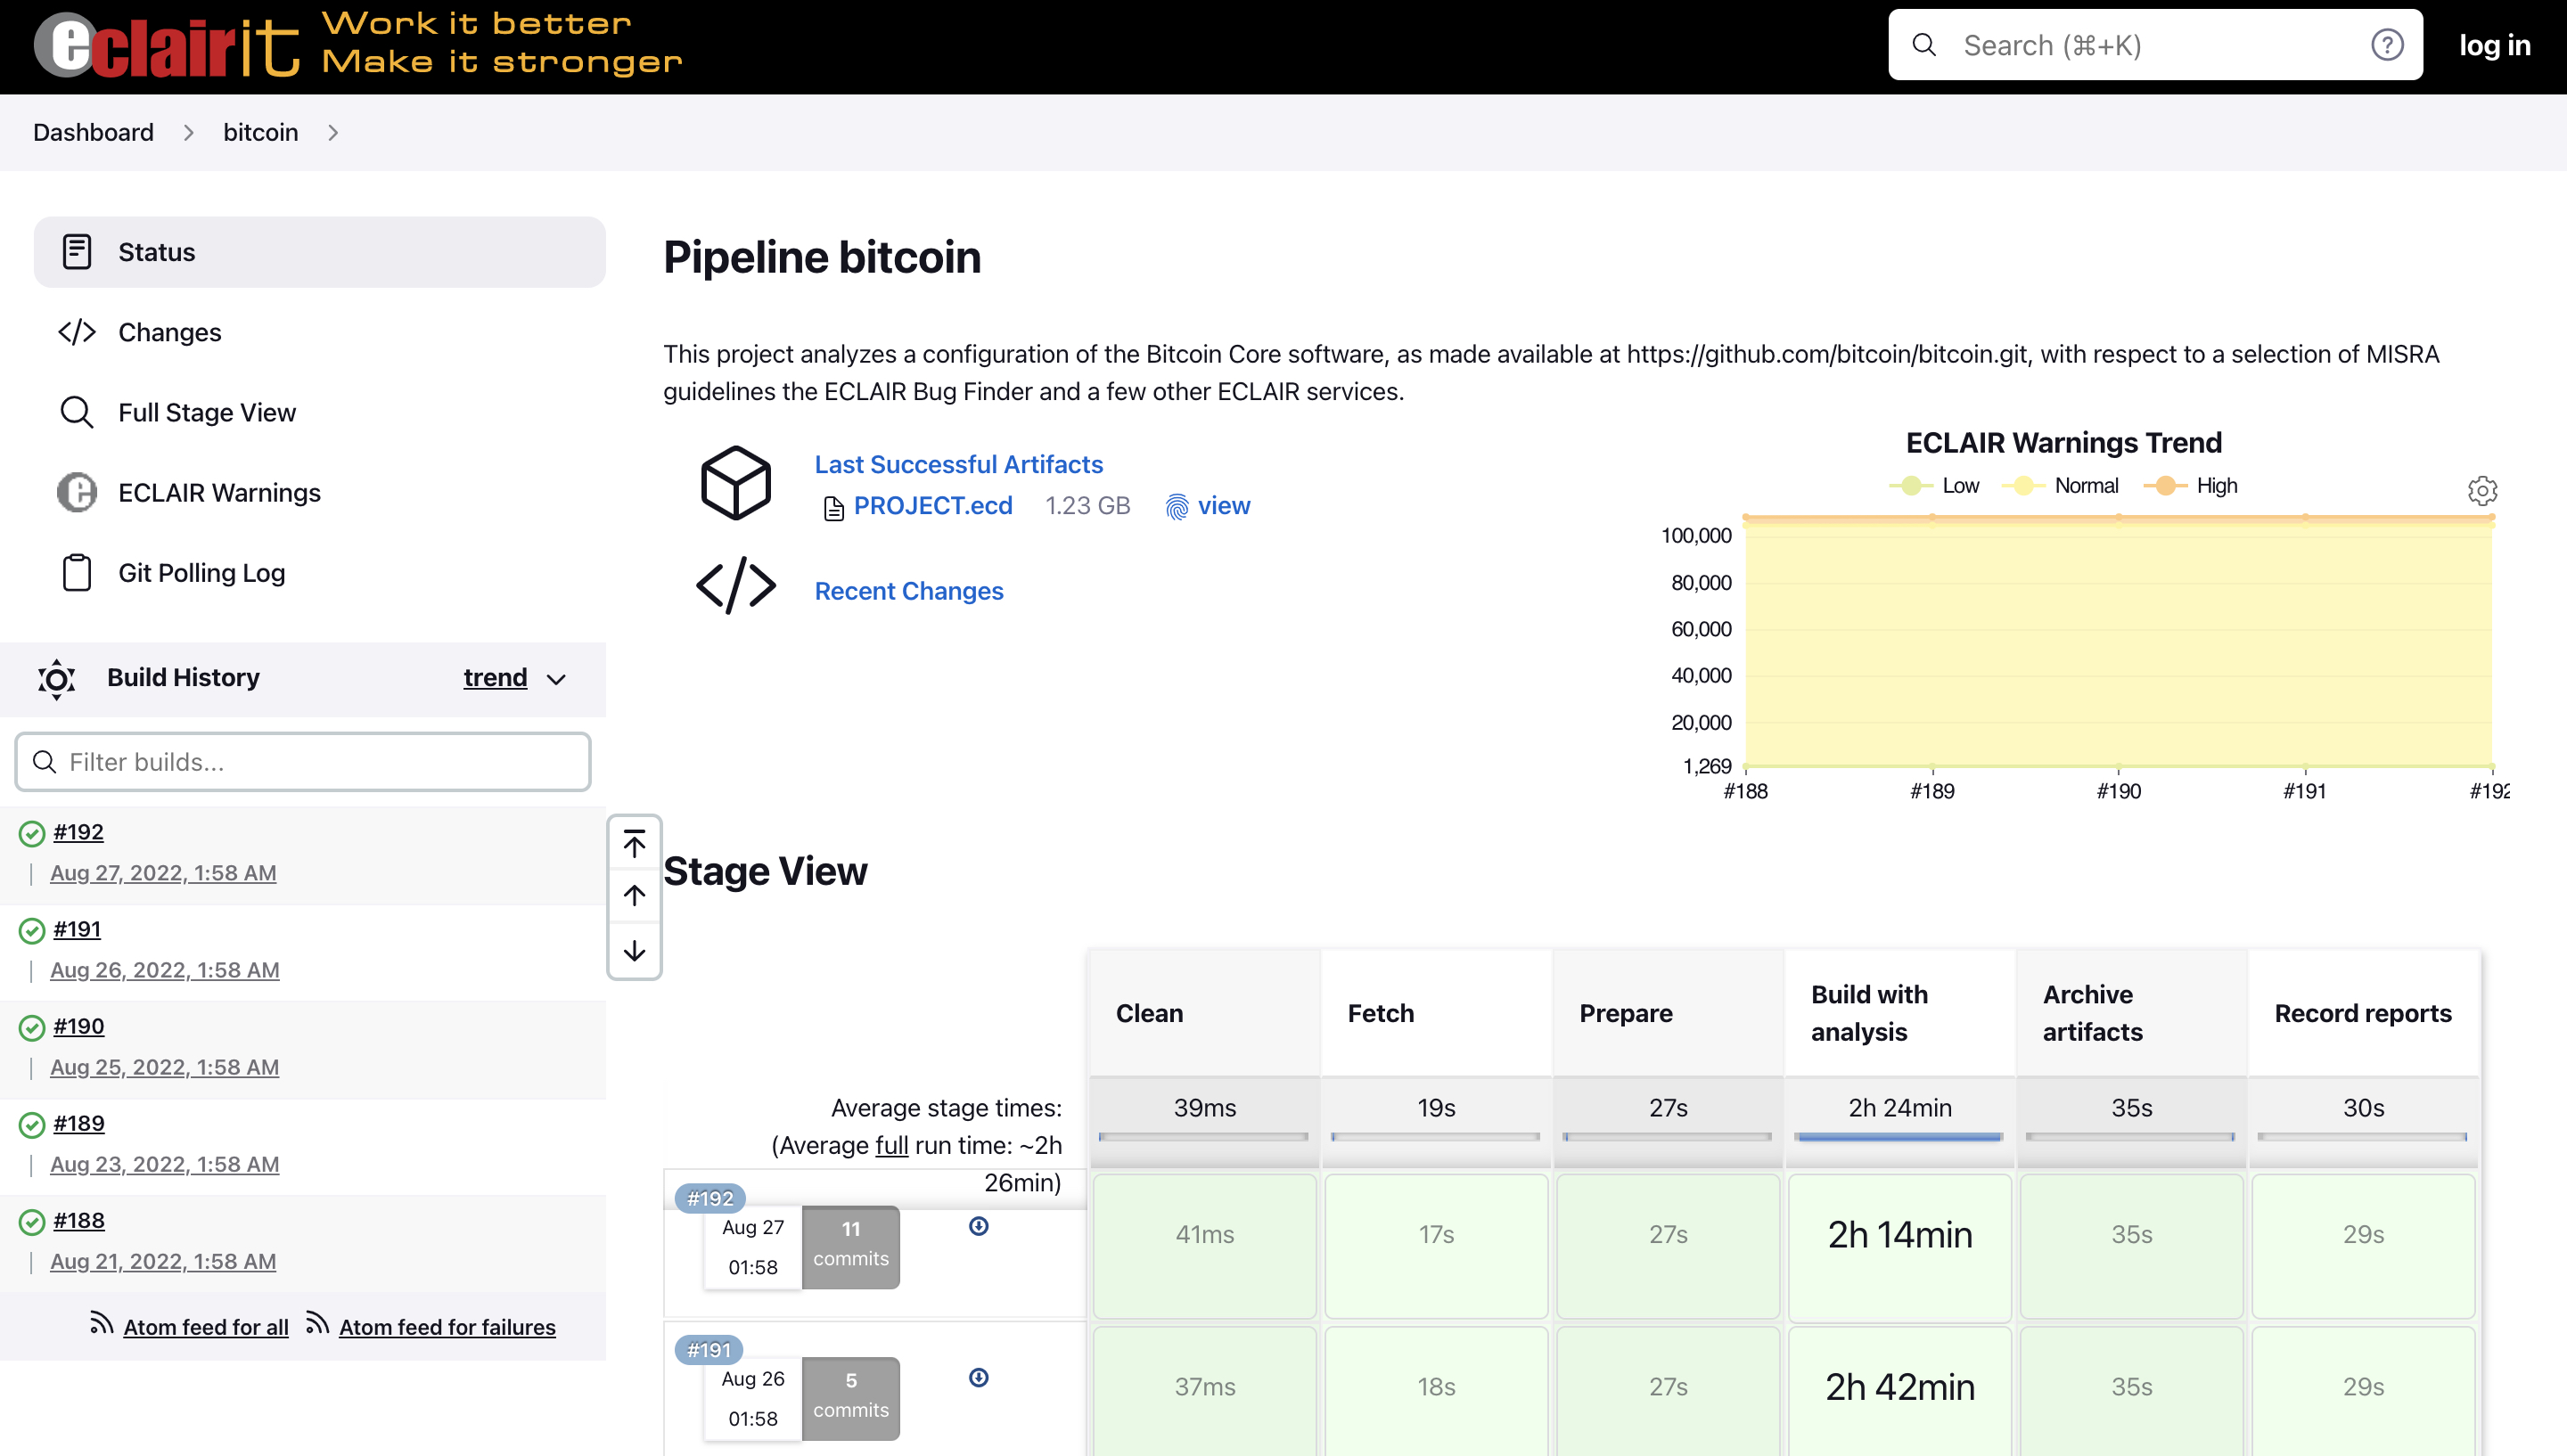
\includegraphics[width=1\textwidth]{Immagini/eclairit.jpg}
	\caption{eclairit.com}
	\label{fig:one}
\end{figure}